\documentclass[12pt]{article}
%\usepackage[swedish]{babel}
%\usepackage[latin1]{inputenc}
\usepackage{graphicx}
\usepackage{fullpage}
\usepackage{pdfpages}
\usepackage{float}
\usepackage{listings}
\usepackage{color}
\title{Report lab 1}
\author{Group 22}
\date{\today}

\setlength{\parindent}{0pt}
\setlength{\parskip}{2ex}

\begin{document}

%\includepdf{Forsattsblad_SigSys.pdf}

\pagebreak

\maketitle

\pagebreak

\tableofcontents

\pagebreak

\section{Introduction}
This is a report for a laboration in the course Digital Signal Processing TSRT78.
The laboration consist of three assignments.
All of them are related to AR models and estimation of them.
The assignments are implemented in Matlab.
Input data for the assignments where collected by recording sounds and importing them into Matlab.
These sounds where then used to complete the assignments.

\section{Whistle}
\subsection{Task}
The first assignment is about measuring the purity of a sound compared to a sine wave. The input data is a recorded whistle and the purity is estimated using harmonic distiortion in the time and frequency domain and an AR-model of second order. The fourier transform of the whistle is shown in figure \ref{forwhis}.

\begin{figure}[H]
\centering
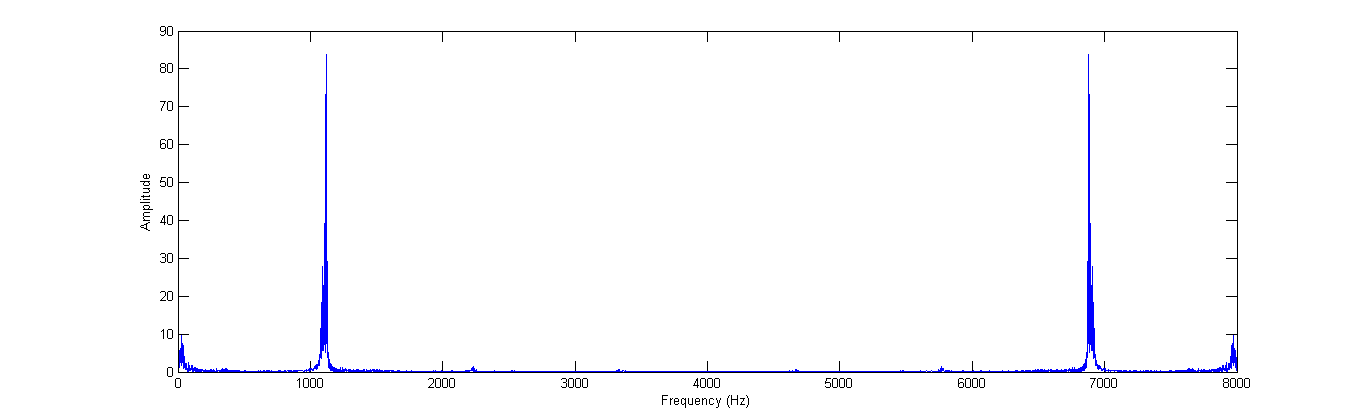
\includegraphics[width=14cm]{Fouriertranswhis.png}
\caption{The fouriertransform of the signal processed in the first assignment\label{forwhis}}

\end{figure}

\subsection{Theoretical overview}

\subsubsection{Energy and harmonic distortion}
A good way to approxiamate the purity of a periodic signal is to calculate the harmonic distorion. It is defined:

\begin{equation}Dist = 1-\frac{E_{dom. freq.}}{E_{tot.}}\end{equation}

The energy $E$ for a signal is defined as

\begin{equation}E=\int_{0}^{T_{L}} \vert y(t)\vert ^2 dt=\frac{1}{2\pi}\int_{\frac{-\pi}{T}}^{\frac{\pi}{T}}\vert Y(\theta)\vert ^2d\theta \end{equation}
%ssjukt fula integraler. bör fixas

where $Y(\theta)$ is the fouriertransform of $y(t)$ and $T_L$ is the length of the signal. Since the signals in this laboratory are timediscrete, the energy can not be calculated this way. The integrals can instead be approximated as a sum of $N$ elements that have the width $T$, where $T$ is the sample period.

\begin{equation}
E=\int_{0}^{T_{L}} \vert y(t)\vert^2 dt\approx T\sum_{n=0}^{N-1}\vert y(n) \vert^2 
\label{A} 
\end{equation}

and

\begin{equation}
E=\frac{1}{2\pi}\int_{\frac{-\pi}{T}}^{\frac{\pi}{T}}\vert Y(\theta)\vert ^2d\theta \approx \frac{2\pi T}{N}\frac{1}{2\pi}\sum_{n=0}^{N-1}\vert Y(\theta) \vert^2=\frac{T}{N}\sum_{n=0}^{N-1}\vert Y(\theta) \vert^2 
\end{equation}

\subsubsection{AR}
\label{ar} 
AR means auto-regressive and is a way of modeling signals. $AR(n)$ is defined as

\begin{equation} 
y(t)+a_1y(t-1)+...a_ny(t-n)=e(t) 
\end{equation}

where $e(t)$ is white noise. In the frequency domain

\begin{equation}
\label{Hfreq}
(1+a_1z^{-1}+..+a_nz^{-1})Y(z)=E(z) \Leftrightarrow H(z) = \frac{1}{(1+a_1z^{-1}+..+a_nz^{-1})}
\end{equation}


With the notation

\begin{equation}
(\varphi(t) =(-y(t-1) ... -y(t-n))^T,\theta = (a_1 ... a_n)^T 
\end{equation}

$y(t)$ can be defined as the linear model

\begin{equation}
y(t)=\varphi^T(t)\theta+ e(t)
\end{equation}

The optimal use of $\theta$ is

\begin{equation}
\hat{\theta}=arg_{\theta}min \frac{1}{N}\sum_{t=1}^{\infty}(y(t)-\varphi^T(t)\theta)^2
\end{equation}

which is given by

\begin{equation}
\hat{\theta}=\left(\sum_{t=1}^N\varphi(t)\varphi^T(t)\right)^{-1}\left(\sum_{t=1}^N\varphi(t)y(t)\right)
\label{enwhis}
\end{equation}

To resample the model to a signal a signal pulse train of white gaussian noise is filtered by the filter consisting of the AR-coeffiecients $\theta$.

An other way of measuring purity than harmonic distortion is to use an AR-model and measure the distance to the poles from the unit circle. A pure sine-wave has its poles on the unit circle and a long distance means an unpure signal.


\subsection{Practical Execution}
The distortion of the signal can be calculated in two different ways. Either the energy of the signal is calculated in the time-domain or in the frequency domain. In this lab both methods are handeled.

The energy for the whole signal in the the time-domain is calculated according to equation \ref{A}. The energy for the dominating frequencies is acquired by filtering the signal with a bandpassfilter with the dominating frequencies in the passband. The dominating frequencies for the whistle can be approximated to 1080-1160 Hz. 

\begin{equation}
E_{tot.} \approx 0.001385, E_{dom. freq.}\approx 0.001314, Dist_{time} = 0.05109
\end{equation}

The energy for the whole signal in the frequency-domain is calculated according to equation \ref{enwhis}. The energy for the dominating frequencies can be approximated with the same sum but over only the dominating frequencies. 

\begin{equation}
E_{tot.} \approx 0.001385, E_{dom. freq.}\approx 0.001337, Dist_{freq.} = 0.03483
\end{equation}

% inse vad som är fel med energin och lös det!


The second order AR-model is calculated as described in section~\ref{ar}.  The AR-model of the whistle has $H(z)$ with roots $z=0.6435 \pm 0.7558i$, both with absolute value $0.9926$. That implies that the whistle is very pure. 

To verify that the AR(2) model is a good choise of estimate, the total error $\lambda$ is computed for different orders of AR-models. This is called the loss-function The total error is 

\[\sum_{k=0}^{N-1}(y(k)-\hat{y})$$

where $y(k)$ is the original function and $\hat{y}$ is the resampled model of the original function.  The results in shown in figure~\ref{whisknee}. A small error is always  a better estimate. A filter with more coefficients is on the other hand more expensive. To obtain a good but still cheap filter a "knee" is searched for in the loss-function. From figure~\ref{whisknee} it is obvious that 2 is the best choice of order.   

\begin{figure}[H]
\centering
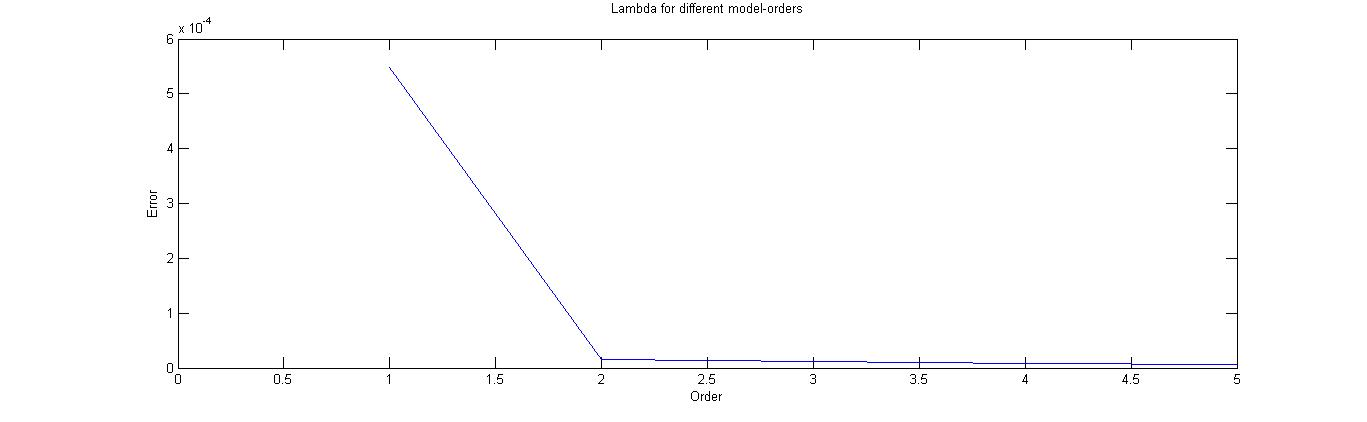
\includegraphics[width=14cm]{whistleknee.jpg}
\caption{The model-errors for different orders of AR-models.\label{whisknee}}
\end{figure}

The spectrum of the signal can also be approximated using welchs method of estimating Power spectral density. The figures \ref{psdwhis} and \ref{psdar2} shows the spectrum of the unparametric recorded whistle and the parametric AR(2)-model. These figures have the axes graded in $\pi \times rad/s$ and not $Hz$ as in figure~\ref{forwhis}. Converting the dominating frequencies from figure~\ref{forwhis} (1080-1160 Hz) to $\pi \times rad/s$ gives the frequencies 0.27-0.29 $\pi \times rad/s$. Both figure~\ref{psdwhis} and figure~\ref{psdar2} also have their most dominating frequencies in that area. Figure~\ref{psdwhis} also have peaks that are multiples of the dominating frequencies. Those are over-tones that are not dealt with when making the AR-model. The over-tones are amplified in figure~\ref{psdwhis} since it uses a logarithmic scale. 

\begin{figure}[H]
\centering
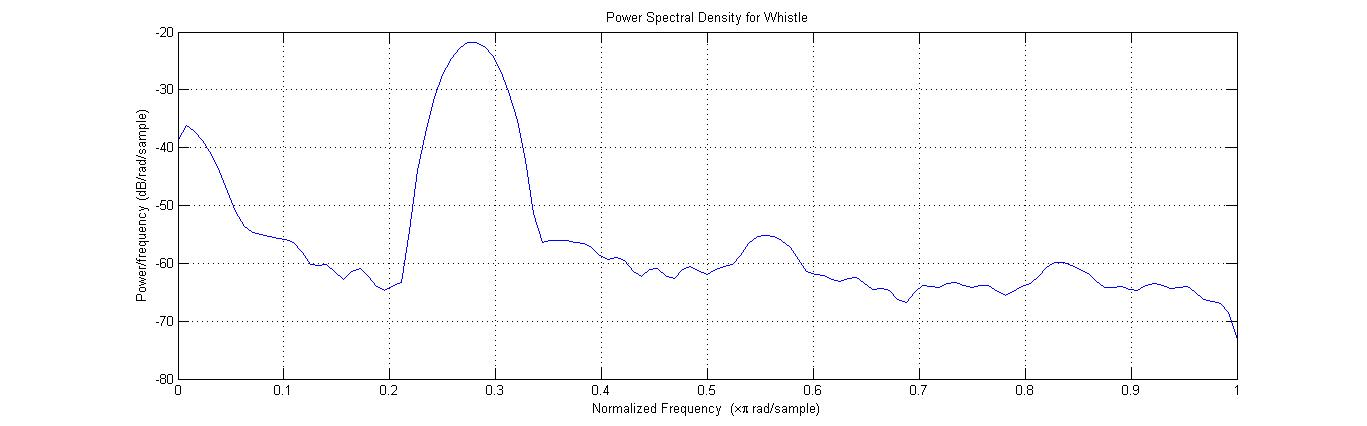
\includegraphics[width=14cm]{psdwhis.jpg}
\caption{The spectrum of the recorded whistle.\label{psdwhis}}
\end{figure}

\begin{figure}[H]
\centering
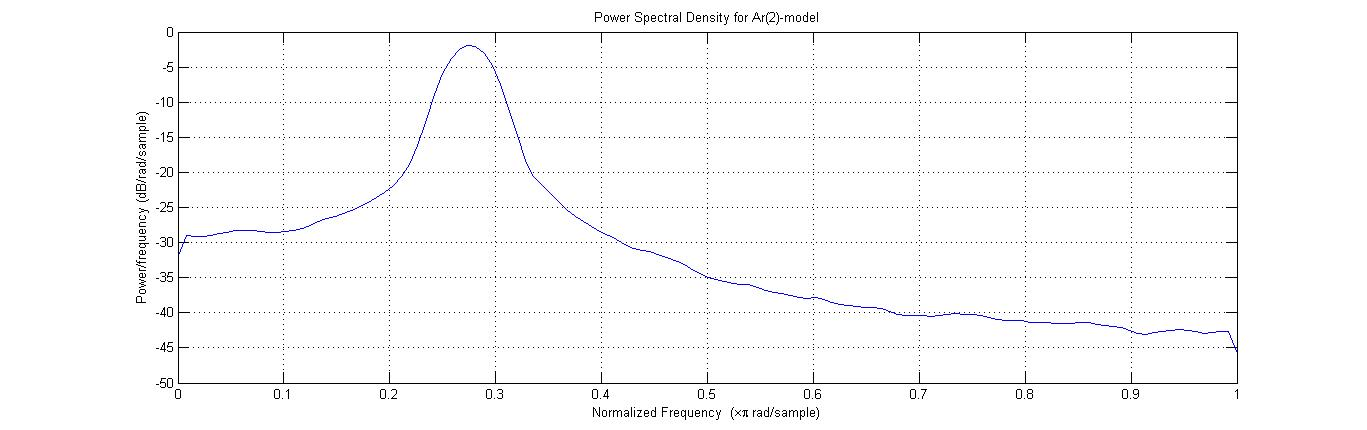
\includegraphics[width=14cm]{psdar2.jpg}
\caption{The spectrum of the AR(2)-model.\label{psdar2}}
\end{figure}


\subsection{Conclusion}
All test of purity of the whistle indicates that the whistle is very pure. Although it contains some overtones. The energies calculated in the frequency domain are almost the same as in the time domain. Since the filter is not ideal and the dominating frequencies are chosen by hand this is as good results as expected. An AR-model of second order is a good estimate of the whistle. It does not model every frequency exactly right but it is really good for the dominating frequencies. 

\section{Vowel}

\subsection{Task}
In this assignment an AR model for a the vowels 'a' and 'o' is to be estimated.
The required order of the model is unknown and to find an appropriate order is part of the assignment.
The estimated models should also be validated and different order models should be compared.

\subsection{Theoretical overview}
An AR model of the sound can be found in the same way as was done in the first assignment.
The problem this time is that a good order for the model must be found.
Different model orders need to be validated and compared.
A good way to do this is splitting the available data into two sets. One set is used to estimate the model and the other set is used for validation.
Now there is a couple of ways of validating that the model order is well chosen.
The ways chosen for this assignment was by calculating the loss function for validation data and by residual covariance plots.

The loss function $W_N$ is the entity that is minimized by the AR-estimation.
Let the loss function depend on n $W_N(n)$ where n is model order.
If the loss function $W_N(n)$ is calculated for the estimation data it will always be less or equal than $W_N(n-1)$.
When the model order increases the model with lower order is contained in the new model.
That means that a higher order model can at least get the same loss function as a lower order model, by just choosing the lower order model.
Since the loss function is minimized the loss function will always be less or equal than a lower order model.
This means that it's hard to use this to choose a good model order.
If the loss function is instead calculated for validation data it can be shown that the loss function has a minimum for the true model order.
This means that the loss function for validation data can be used to estimate model order.

The residual covarince approach for model validation exploits the fact that an AR model is filtering white noise.
This means that if the inverse filter is applied to validation data the result should be white noise.
Let this inverse filtered data be $\epsilon(t)$ then $R_{\epsilon \epsilon}(\tau) = \lambda\delta(t)$.
Since $\epsilon(t)$ is white noise $R_{\epsilon y}(\tau) = E\epsilon(t) y(t-\tau) = 0$ for $\tau > 0$.
This can then be used for validation of models.
The estimation of $R_{\epsilon y}(\tau)$ should not be to far from zero.

\subsection{Practical Execution}
To get data to use in the assignment two sounds are recorded. One with an a-sound and one with an o-sound.
The recordings are each two seconds long.
These files are then imported into Matlab and the means of the signals are removed.
The signals are then split into estimation and validation data.
The DFT of the signal is then generated and plotted.
DFTs can be used to get a rough estimate of model order by counting the number of peaks in them.
Each pair of complex-conjugated poles of the AR model will create a peak in the model spectrum.
This means that counting the peaks in the spectrum and multiplying by two will be an estimate of the model order.
These DFTs are presented in figure \ref{vowel_DFT}.
The a-sound has three more prounounced peaks that are about the same height, there are also a few smaller peaks at higher frequencies.
The o-sound has one peak that are higher than the others then there are two more peaks that are a bit smaller.
This is an indication that the a-sound probably needs a higher order model than the o-sound.

After this an AR-model is estimated for orders 1-20 and the loss function of the validation data is plotted with respect to model order.

The result can be seen in figure \ref{loss_function}. 

The o-sound has a clear "knee" at order 2 and an at least local minima at order 5.
This suggest that the AR of order 2 probably is sufficient but orders up to 5 will probably improve the model.
Higher model orders than 5 seems unnecessary.

The order of the a-sound is harder to estimate.
This plot has no clear "knee" and the estimation seems to be getting better and better when the model order increases.
The loss function for the a-sound is also larger than for the o-sound.
This is an indication that the model for the a-sound might not be that good.
After order 10 the loss functions seems to be more or less horizontal so this might be a good order estimate.

When this is done the models should be validated.
First $\epsilon(t)$ is calculated and checked for whiteness.
This is done by checking the probability of a sign change for between $\epsilon(t)$ and $\epsilon(t+1)$.
The results is

\begin{tabular}{l|l|l|l|l|l|l|l|l|l|l}
  \hline
  Model order & 1 & 2 & 3 & 4 & 5 & 6 & 7 & 8 & 9 & 10 \\
  A-sound & 0.344 & 0.657 & 0.439 & 0.472 & 0.462 & 0.474 & 0.485 & 0.468 & 0.429 & 0.502 \\
  O-sound & 0.122 & 0.520 & 0.567 & 0.595 & 0.539 & 0.554 & 0.551 & 0.542 & 0.555 & 0.552 \\
\end{tabular}

Both the signals seems to have models that change sign with about 50 \% chance when the model order is higher than 2.
For the o-sound even the second order model seems to behave well.

After this is done another test is used on the same $e(t)$.
$R_{ey}$ the residual covariance is estimated and then plotted for model orders 1-4.
The result is in figures \ref{res_cov_a} and \ref{res_cov_o}.
Notice that the plot for model order 1 is scaled differently than the rest.
A plot that is close to zero means that the model is good.
Here it seems that model order should be a bit higher for the a-sound than for the o-sound.
The o-sound seems fine for model order 4.
The a-sound still is a bit above zero and there is some positive correlation with the input signal.
This is also true for higer order models of the a-sound.
This is not that much though.

Now the estimations can be tested by generating sounds from the models.
This is done by creating a pulse train with the same period as the recorded sounds and then filtering it with the filter created in the AR estimation.
The period is easy to find in the DFTs of the recordings.
The amplitude of the pulse train is found by simple testing until the generated sounds has a reasonable volume.
The generated files sounds a bit syntetic but you can distinguish the a-sound from the o-sound.

\subsection{Conclusion}

With all of this a reasonable model order for the o-sound seems to be 4.
This model order has done well on all the validation methods it has been tested with.
The model order for the a-sound should probably be a bit higher although a good conclusion is hard to reach.
A model order of 8 to 10 is probably good.
It seems that it is possible to create reasonably good models for the vowels a and o.

\begin{figure}[H]
  \centering
  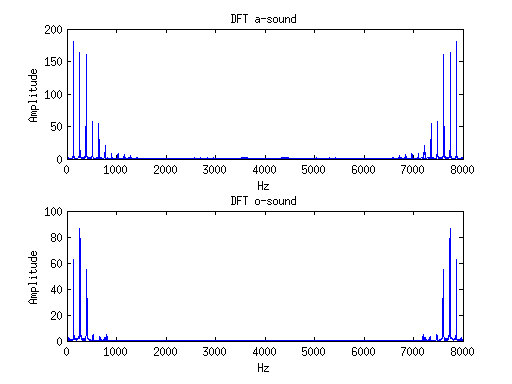
\includegraphics[width=14cm]{vowel_fft.png}
  \caption{
    \label{vowel_DFT}
    DFTs of the vowels.}
\end{figure}

\begin{figure}[H]
  \centering
  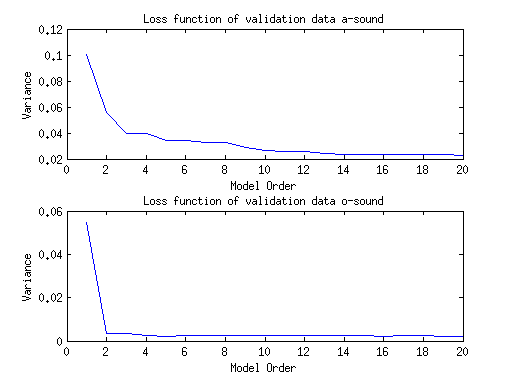
\includegraphics[width=14cm]{loss_function_validation.png}
  \caption{
    \label{loss_function}
    The loss function as a function of model order}
\end{figure}

\begin{figure}[H]
  \centering
  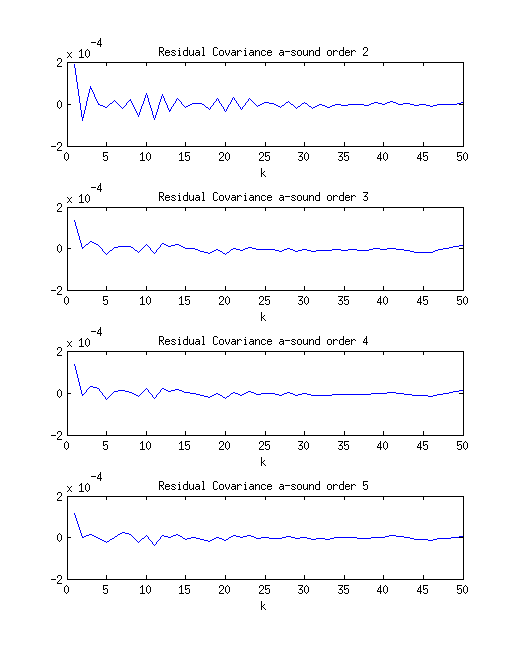
\includegraphics[width=14cm]{residual_covariance_a.png}
  \caption{The residual covariance of different model orders for the a-sound\label{res_cov_a}}
\end{figure}

\begin{figure}[H]
  \centering
  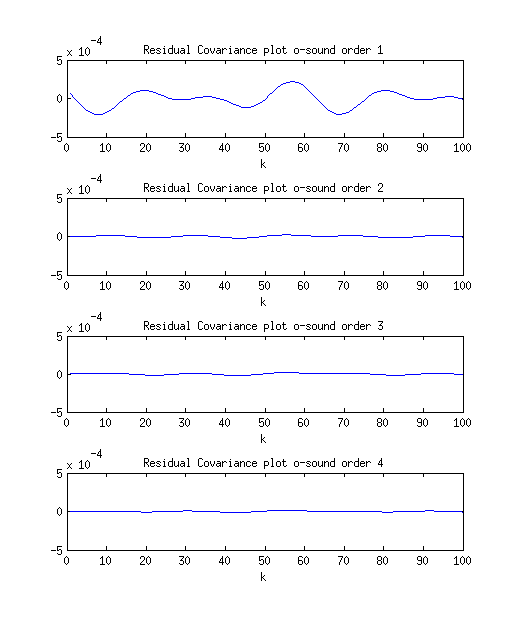
\includegraphics[width=14cm]{residual_covariance_o.png}
  \caption{The residual covariance of different model orders for the o-sound\label{res_cov_o}}
\end{figure}

\section{Sentence}

\subsection{Task}
In the last assignment an AR(8)-model is used to estimate a recorded sentence. AR-models of 8th order are used in GSM encoding in cellphones.

\subsection{Theoretical overview}
\label{Theo}
The theory in this assignment is mostly the same as in the first two assignments.
The biggest difference is that the sentence is divided into segments of 160 samples each. 
For each segment an AR-model is calculated. 
To decide the optimal amplitude $A$ and period $D$ for the input pulse train of each segment the covariance function for the modeled signal is used. 
The square root of the maximum of the auto covariance function is the amplitude of the pulse train and the period of the pulse train is the time where the auto covariance function reaches its maximum. 
To be sure to get a stable filter unstable poles must be made stable. 
This can be done by mirroring them in the unit circle. 
Also in every segment the mean of the original signal is removed, since the estimation assumes a mean zero.  

\subsection{Practical Execution}
The estimation is done according to the description in section~\ref{Theo} but to get a better result some modifications are made.
Instead of using a pure pulse train as input, noise is added to it everywhere.
The following noise is input $u(t)$ to the filter.
$\lambda$ is the mean of the auto covariance function of the segment $N_{num}$ are the number of samples in the segment and $A$ and $D$ are the same as described in section~\ref{Theo}. 

\[u(t)= e_1(t)+e_2(t)sum_{k=0} ^N \delta(t-kD),
e_1(t)\sim N(0,\lambda),e_2(t)\sim N(0,\sqrt{N_{num}A/D}$$

\section{Conclusion}
An eight order AR-model can model a voice so good that it can be used in a cellphone. However it has to be modified to be really good. The reason that AR is used is that it compresses the signal. The whole signal is not sent but only the coefficients in $\theta$. In this case where an eight order AR-model is used for an interval of 160 samples the compression is 95\% (8/160 = 0.05). 




%\begin{figure}[H]
%  \centering
%  \includegraphics[width=14cm]{flow_chart.png}
%  \caption{Flow chart of Slotted ALOHA simulation.}
%\end{figure}


\clearpage
\section{Source Code}
\definecolor{dkgreen}{rgb}{0,0.6,0}
\definecolor{gray}{rgb}{0.5,0.5,0.5}
\definecolor{mauve}{rgb}{0.58,0,0.82}
\lstset{
  title=\lstname,
  basicstyle=\footnotesize\ttfamily,
  keywordstyle=\color{blue},          % keyword style
  commentstyle=\color{dkgreen},       % comment style
  stringstyle=\color{mauve},         % string literal style
  showstringspaces=false,         % underline spaces within strings
}
\lstinputlisting[language=Matlab]{vowel.m}
\lstinputlisting[language=Matlab]{sentence.m}
\end{document}

